\section{Literaturverzeichnis der Literaturrecherche der 3D-Netze}
\label{Literaturverzeichnis der Literaturrecherche}

\begin{list}{}{\leftmargin=1.27cm \itemindent=-1.27cm \itemsep=0.5em}

\item Ambrosini, Y. \& Merz, L. (2022). \textit{Deformationsmessungen Schlipf, Riehen BS} [Bachelor-Thesis, Fachhochschule Nordwestschweiz]. \url{https://www.fhnw.ch/de/architektur-bau-geomatik/studium/angebot/studiengaenge/bachelor-in-geomatik/bachelorthesen/bachelor-thesis-2022/bth22_01.pdf}

\item Banyai, L. (2011, 18.--22. Mai). \textit{Rigorous 3D integrated adjustment of GPS baselines, geodetic total station and levelling measurements} [Konferenzbeitrag]. FIG Working Week 2011: Bridging the Gap between Cultures, Marrakesch, Marokko. \url{https://www.fig.net/resources/proceedings/fig_proceedings/fig2011/papers/ts08f/ts08f_banyai_5363.pdf}

\item França, R. M. de, Klein, I. \& Veiga, L. A. K. (2021). The influence of the deflection of the vertical on geodetic surveys in Brazil. \textit{Boletim de Ciências Geodésicas, 27}(spe), Artikel e2021020. \url{https://doi.org/10.1590/s1982-21702021000s00020}

\item GeoConnexion. (2016, 22. März). \textit{New Leica LS15 digital level provides industry-leading accuracy}. \url{https://www.geoconnexion.com/publication-articles/new-leica-ls15-digital-level-provides-industry-leading-accuracy}

\item Leica Geosystems. (o.\,J.-a). \textit{Leica Nova TS60} [Produktseite]. Abgerufen am 7. Oktober 2026, von \url{https://leica-geosystems.com/products/total-stations/robotic-total-stations/leica-nova-ts60}

\item Leica Geosystems. (o.\,J.-b). \textit{Meeting in the middle} [Fallstudie]. Abgerufen am 20. November 2026, von \url{https://leica-geosystems.com/case-studies/heavy-construction/meeting-in-the-middle}

\item Leica Geosystems. (2025). \textit{Leica GS18 data sheet} [Datenblatt]. \url{https://bynder.hexagon.com/m/47f3f231ddd904d6/original/Leica-GS18-DS-949487-0422-en-LR.pdf}

\item Möser, M. (Hrsg.). (2016). \textit{Handbuch Ingenieurgeodäsie: Ingenieurbau} (2., neu bearb. und erw. Aufl.). Wichmann.

\item Niemeier, W. (2008). \textit{Ausgleichungsrechnung: Statistische Auswertemethoden} (2., überarb. und erw. Aufl.). de Gruyter. \url{https://doi.org/10.1515/9783110206784}

\item Suurmäki, H., Schüler, T., Klügel, T., Kallio, U., Marila, S., Mähler, S., Poutanen, M. \& Saari, T. (2022). Datum problem handling in local tie surveys at Wettzell and Metsähovi. In \textit{International Association of Geodesy Symposia}. Springer. \url{https://doi.org/10.1007/1345_2022_155}

\item Bundesamt für Landestopografie swisstopo. (o.\,J.). \textit{LTOP: Präanalyse- und Ausgleichungssoftware für geodätische Netze}. Abgerufen am 7. Oktober 2026, von \url{https://www.swisstopo.admin.ch/de/geodaetische-software-ltop}

\item Bundesamt für Landestopografie swisstopo. (2004). \textit{Geoidmodell der Schweiz CHGeo2004} [Datensatz]. \url{https://www.swisstopo.admin.ch/de/geoid}

\item Vasi, S. \& Meyenberg, S. (2014). \textit{Deformationsmessung Strain-Zone Le Pont (Jura Decke)} [Bachelor-Thesis, Fachhochschule Nordwestschweiz FHNW]. \url{https://www.fhnw.ch/de/studium/architektur-bau-geomatik/bachelor-studiengang-geomatik/bachelor-thesis-2014/media/bth14-01.pdf}

\item Weber, F. (2014). \textit{Ceneri-Basistunnel -- Portalnetz Zwischenangriff Sigirino} [Bachelor-Thesis, Fachhochschule Nordwestschweiz]. \url{https://www.fhnw.ch/de/studium/architektur-bau-geomatik/bachelor-studiengang-geomatik/bachelor-thesis-2014/media/bth14-04.pdf}

\item Willi, D., Borlat, E. \& Deillon, Y. (2024, 15. Mai). \textit{Neues Höhensystem der Schweiz: Einleitung, Stand, Roadmap} [Präsentation]. GEOSummit 2024, Olten. \url{https://swiss-height-system.heig-vd.ch/wp-content/uploads/2024/05/2024-05-15-GeoSummit.pdf}

\end{list}

\section{Deklaration von KI}
\label{Deklaration von KI}

\begin{table}[h]
\centering
\small
\begin{tabularx}{\textwidth}{>{\raggedright\arraybackslash}p{3.2cm} X >{\raggedright\arraybackslash}p{3.2cm} >{\raggedright\arraybackslash}p{2.4cm}}
\toprule
\textbf{KI-basiertes Hilfsmittel} & \textbf{Einsatzform} & \textbf{Betroffene Teile der Arbeit} & \textbf{Datum} \\
\midrule
Claude Opus 5.5 (Anthropic) & Überprüfung und Korrektur der Zitierweise sowie der Darstellung der Links & Gesamte Arbeit, Quellenverzeichnis & November 2026 \\
Claude Opus 5.5 (Anthropic) & Alphabetische Sortierung des Literaturverzeichnisses & Literaturverzeichnis & Oktober 2026 \\
Claude Opus 5.5 (Anthropic) & Verständliche Erklärung des Inhalts & Kapitel 1.4 & Oktober 2026 \\
Claude Opus 5.5 (Anthropic) & Rechtschreibprüfung & Gesamte Arbeit & Oktober 2026 \\
\bottomrule
\end{tabularx}
\caption{Dokumentation des KI-Einsatzes}
\end{table}

\section{Anhang}
\label{app:anhang}

\begin{enumerate}
  \item \hyperlink{pdf:ltop}{\texttt{LTOP-Bericht\_TPS-Messungen}}
\end{enumerate}

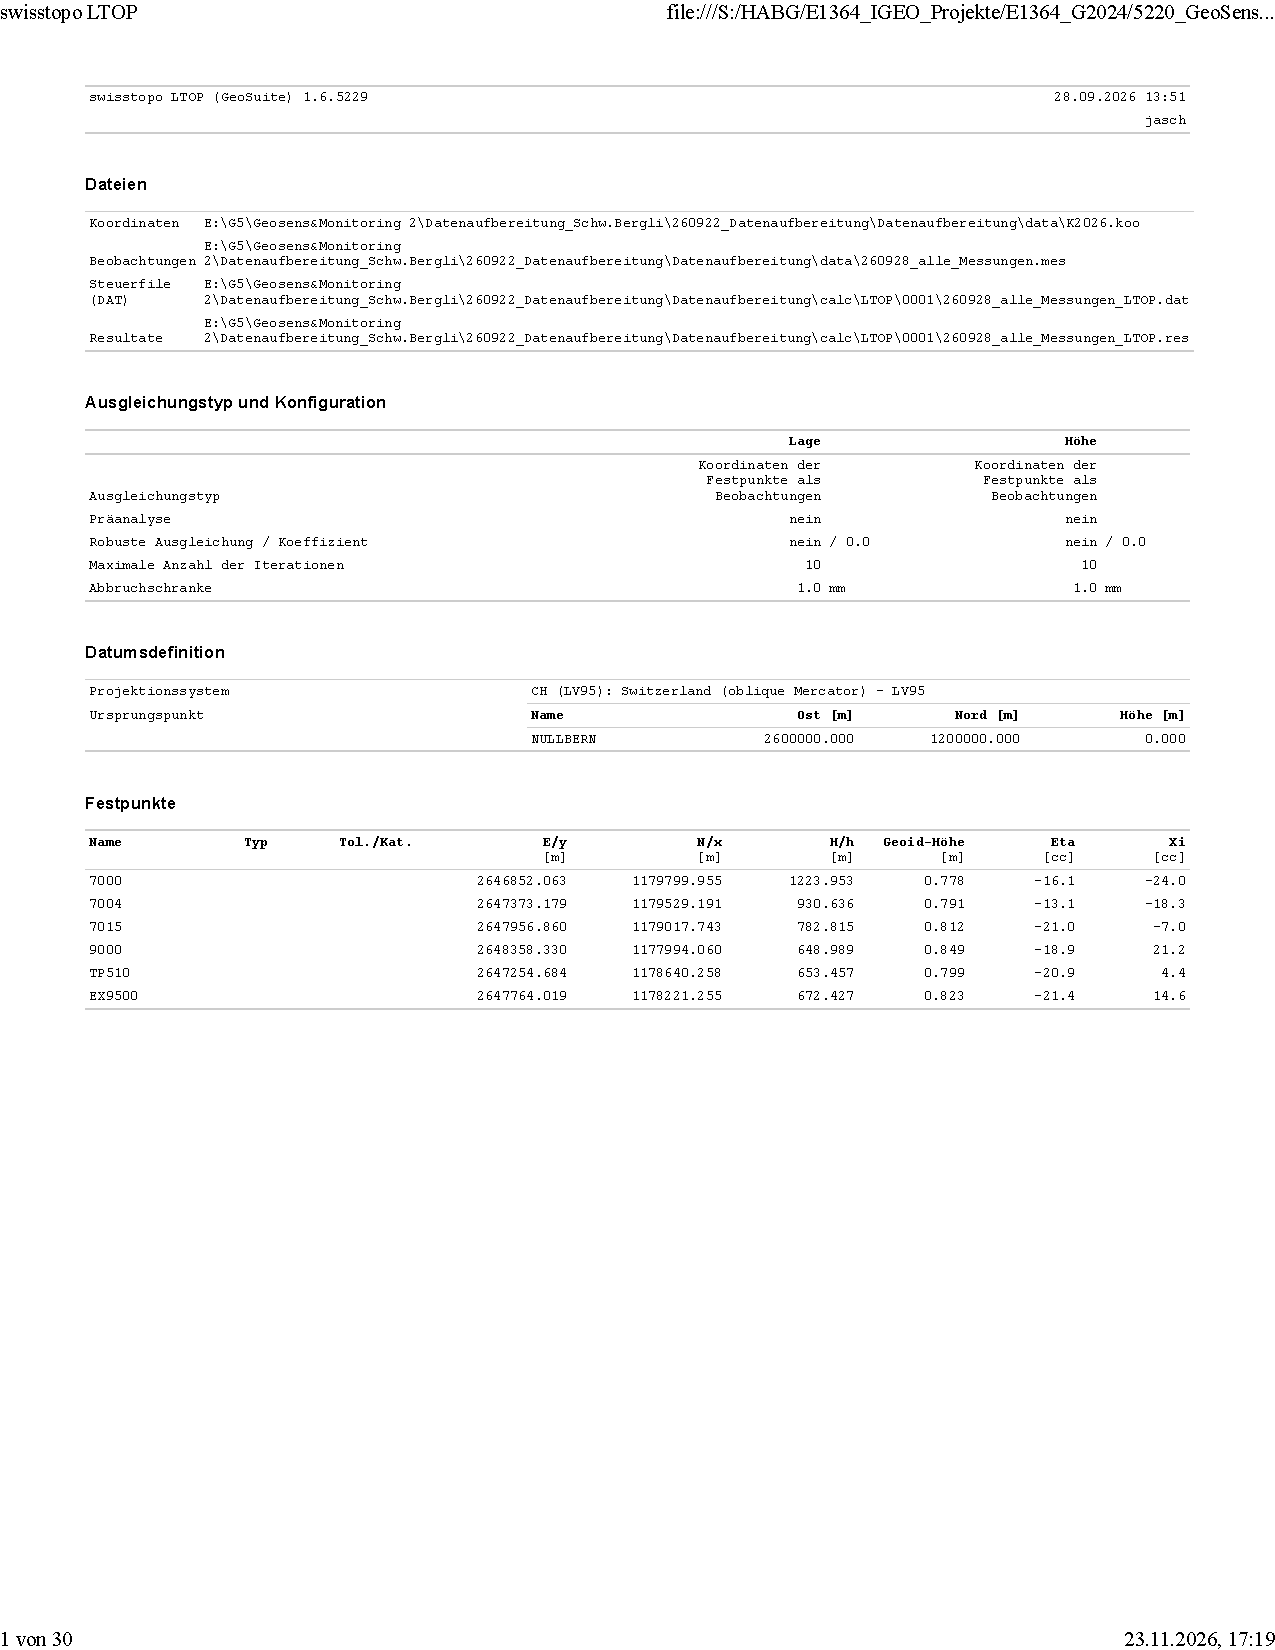
\includepdf[pages=1, pagecommand={\hypertarget{pdf:ltop}{}}]{anhang/LTOP_TPS-Messungen.pdf}
\includepdf[pages=2-, pagecommand={}]{anhang/LTOP_TPS-Messungen.pdf}

\clearpage